\documentclass[conference]{IEEEtran}
\usepackage{cite}
\usepackage{amsmath,amssymb,amsfonts}
\usepackage{algorithmic}
\usepackage{graphicx}
\usepackage{textcomp}
\usepackage{xcolor}
\usepackage{booktabs}
\usepackage[caption=false,font=footnotesize]{subfig}
\usepackage{dblfloatfix}
\usepackage{hyperref}

\graphicspath{{figures/}{./}{artifacts/stitch_design/}}

\hypersetup{
    colorlinks=true,
    linkcolor=black,
    citecolor=black,
    urlcolor=blue
}

\begin{document}

\title{Generative AI Assignment 1: Restoration Studio and Style-Conditioned Face-to-Sketch Synthesis: A Comparative Study of Autoencoding, Adaptive Routing, and Adversarial Generation}

\author{\IEEEauthorblockN{Muhammad Usman Bari (23i-0680)}
\IEEEauthorblockA{\textit{Section A} \\
\textit{Department of Computer Science} \\
\textit{Generative AI --- Assignment 1} \\
\textit{GitHub Repository:} \url{https://github.com/UsmanBari/genai-restoration-studio} \\
\textit{Demonstration Video:} \url{https://youtu.be/AfU6j4_NIp0}}}

\maketitle

\begin{abstract}
Image restoration and paired image-to-image synthesis represent foundational challenges in generative computer vision, requiring distinct balances between structural fidelity, domain adaptability, and computational efficiency. This paper presents the end-to-end design, optimization, comparative empirical evaluation, and containerized deployment of four distinct generative systems developed for Generative AI Assignment 1. 
First, for multi-corruption image restoration on the Oxford-IIIT Pet dataset, we investigate a \textit{Universal Denoising Autoencoder} operating under strict bottleneck compression ($6.0\times$) with a learned high-resolution gated skip connection. 
Second, we evaluate a \textit{Hard-Routing Restoration System} combining an ultra-lightweight 4-class convolutional corruption classifier ($99.95\%$ test accuracy) with three dedicated specialist autoencoders and an exact identity bypass for clean images, lifting mean restoration performance by $+10.34\text{ dB}$ over the universal baseline. 
Third, to mitigate sharp boundary failures and enable differentiable multi-expert collaboration, we construct a \textit{Soft Mixture-of-Experts (MoE)} architecture with temperature-scaled gating ($\tau=0.50$), achieving strict restoration improvements over Hard Routing across all active degradation types ($+1.13\text{ dB}$ on salt-and-pepper, $+1.27\text{ dB}$ on Gaussian blur, and $+0.71\text{ dB}$ on rectangular occlusion), and an overall test set mean of $40.53\text{ dB}$ PSNR / $0.858$ SSIM across $3,669$ test instances (noting that the composite mean reflects near-lossless floating-point identity routing on the $10\%$ clean test partition). 
Fourth, for paired face-to-sketch generation on the FS2K benchmark ($2,104$ pairs across three distinct styles), we develop a style-conditioned conditional Generative Adversarial Network (cGAN) incorporating a 5-stage U-Net generator with learned style embeddings and a $70\times 70$ PatchGAN discriminator ($16.24\text{ dB}$ PSNR, $0.521$ SSIM, $0.0993$ L1 error), accompanied by an empirical investigation into early discriminator dominance dynamics. 
Finally, all seven neural networks are exported to Open Neural Network Exchange (ONNX) format and integrated into a production, torchless FastAPI and React interactive studio running via Docker Compose with sub-150 ms server-side CPU inference latencies.
\end{abstract}

\begin{IEEEkeywords}
Image Restoration, Denoising Autoencoders, Corruption Classification, Mixture-of-Experts, Soft Routing, Conditional GAN, pix2pix, FS2K Dataset, ONNX Runtime, Containerized Deployment.
\end{IEEEkeywords}

\section{Introduction and Related Work}
\IEEEPARstart{I}{mage} restoration aims to recover high-fidelity visual targets from corrupted observations, addressing degradations such as impulsive noise, spatial frequency attenuation, and structured occlusions. In real-world computer vision pipelines, image degradations rarely appear in isolation or under known parameterizations. Consequently, generative models must either learn an invariant shared representation across heterogeneous corruptions or dynamically adapt their internal computational graph to match the specific degradation present in the input. Simultaneously, paired image-to-image synthesis tasks—such as translating facial photographs into artist-styled pencil sketches—require mapping across disparate visual modalities while adhering strictly to user-conditioned stylistic parameters.

\subsection{Evolution of Image Restoration Architectures}
Early convolutional approaches to image restoration relied on deep feed-forward networks trained on single degradation types, such as DnCNN \cite{zhang2017beyond} for Gaussian denoising. While effective within their narrow domain, single-task models fail catastrophically when exposed to unmodeled corruptions. To address multi-degradation settings, modern approaches have diverged along three distinct architectural paradigms:
\begin{enumerate}
    \item \textbf{Universal Shared-Representation Autoencoders:} Single networks trained across all degradation types simultaneously. While computationally straightforward, universal autoencoders suffer from capacity sharing tradeoffs: high-frequency texture reconstruction on clean or blurred inputs often interferes with the spatial filtering required for salt-and-pepper noise and the generative hallucination demanded by rectangular occlusions.
    \item \textbf{Classify-and-Route (Hard Routing) Pipelines:} Two-stage systems where an upfront classifier predicts the corruption label and directs the input to an isolated, independently trained specialist network \cite{yu2018crafting}. This paradigm prevents negative cross-task gradient interference and enables an exact identity bypass on clean images, but it remains brittle to classification mistakes and cannot blend specialist capabilities.
    \item \textbf{Differentiable Mixture-of-Experts (MoE):} Dynamic architectures in which a gating network computes continuous routing weights over multiple specialized sub-networks, taking inspiration from modular neural architectures in natural language processing and vision transformers \cite{shazeer2017outrageously, eigen2014learning}. Soft MoE allows end-to-end gradient flow, enabling specialists to collaborate on ambiguous, compound, or boundary degradation states.
\end{enumerate}

\subsection{Conditional Generative Adversarial Networks for Paired Synthesis}
In paired cross-domain translation, the pix2pix framework established by Isola et al. \cite{isola2017image} demonstrated that combining an adversarial loss with a pixel-level L1 reconstruction penalty forces a U-Net generator to produce sharp, plausible high-frequency details. For style-conditioned facial sketch synthesis, the FS2K benchmark introduced by Fan et al. \cite{fan2022facial} poses unique challenges: paired sketches exhibit significant stylistic variation (varying from delicate pencil cross-hatching to heavy artistic shading and graphic caricature outlines) across a non-uniform distribution of training and test subjects. Incorporating categorical style conditioning directly into the generative and discriminative latent spaces is critical to prevent mode collapse and style ambiguity.

\subsection{Contributions of this Work}
This paper presents a unified, reproducible research investigation spanning the theoretical formulation, empirical optimization, diagnostic failure analysis, and production deployment of four generative vision tasks. The primary contributions include:
\begin{itemize}
    \item \textbf{Bottleneck vs. Skip Justification in Universal Autoencoders:} We document the empirical failure of overly compressed ($4\times 4$) bottlenecks ($17.64\text{ dB}$ PSNR) and demonstrate that an $8\times 8\times 96$ bottleneck ($6.0\times$ compression) combined with a learned, high-resolution Gated Skip Connection resolves spatial underfitting while preserving strict denoising constraints ($29.20\text{ dB}$ clean, $22.51\text{ dB}$ overall).
    \item \textbf{Quantitative Comparison of Hard Routing vs. Soft MoE:} Across a strictly isolated, deterministic test set of $3,669$ Oxford-IIIT Pet images, we establish that Hard Routing delivers a $+10.34\text{ dB}$ gain over Universal modeling, while Soft MoE further improves restoration across every real degradation type ($+1.13\text{ dB}$ S\&P, $+1.27\text{ dB}$ blur, $+0.71\text{ dB}$ occlusion) through continuous collaborative gating.
    \item \textbf{Diagnostic Analysis of Adversarial Dominance in FS2K cGAN:} We report the full training dynamics of style-conditioned cGAN training, documenting the empirical phenomenon of early discriminator dominance ($91$--$94\%$ accuracy) and its direct visual consequence (soft, painterly shading rather than sharp line art), alongside baseline comparisons against All-White, Mean-Sketch, and Grayscale benchmarks.
    \item \textbf{Torchless Production Web Studio:} We deploy all seven trained models via CPU ONNX Runtime within an isolated FastAPI backend and React/Tailwind frontend orchestrated by Docker Compose, verifying real-time sub-150 ms latencies and analyzing empirical out-of-distribution (OOD) domain shifts when pet-restoration models encounter human portrait inputs.
\end{itemize}

\section{Dataset Preparation and Runtime Corruption Engine}
Rigorous, reproducible evaluation of generative restoration and cross-domain synthesis requires deterministic data pipelines and controlled corruption models. We utilize two benchmark datasets: the Oxford-IIIT Pet dataset \cite{parkhi2012cats} for Tasks 1--3 and the FS2K Facial Sketch dataset \cite{fan2022facial} for Task 4.

\subsection{Oxford-IIIT Pet Dataset Pipeline (Tasks 1--3)}
The Oxford-IIIT Pet dataset comprises 7,349 images across 37 cat and dog breeds. In this work, category labels are omitted, and clean RGB images serve as ground-truth reconstruction targets. All images are converted to 3-channel RGB and resized to $128 \times 128$ resolution using bilinear interpolation.
\begin{enumerate}
    \item \textbf{Data Partitioning:} The official development partition (\texttt{trainval.txt}) is divided into an 80\% training set ($2,944$ images) and a 20\% validation set ($736$ images) using random seed 42. The official test set ($3,669$ images from \texttt{test.txt}) is held strictly isolated and evaluated only during final benchmarking.
    \item \textbf{Breed Casing and Invariant Resolution:} To prevent file-resolution errors stemming from Oxford Pet naming conventions (where cat breeds are capitalized, e.g., \texttt{Bengal\_96.jpg}, while dog breeds are lowercase, e.g., \texttt{pug\_60.jpg}), dataset loaders implement case-insensitive fallback resolution, ensuring byte-level consistency across operating systems.
\end{enumerate}

\subsection{Runtime and Deterministic Corruption Configurations}
To prevent disk storage bloat and avoid overfitting to static noise patterns, corruptions are applied dynamically during training within the PyTorch \texttt{\_\_getitem\_\_} DataLoader pipeline. For every clean image $x \in [0, 1]^{3 \times 128 \times 128}$, one of four input conditions is sampled with uniform probability ($p = 0.25$):
\begin{itemize}
    \item \textbf{Clean ($y=0$):} The original image is passed unmodified: $x_{\text{corrupt}} = x$.
    \item \textbf{Salt-and-Pepper Noise ($y=1$):} A noise fraction $p_{\text{sp}} \sim \mathcal{U}(0.02, 0.15)$ is sampled. Selected pixels are replaced with $0.0$ (black) or $1.0$ (white) with equal probability.
    \item \textbf{Gaussian Blur ($y=2$):} A kernel size $k \in \{3, 5, 7\}$ is chosen uniformly, and the standard deviation is sampled as $\sigma \sim \mathcal{U}(0.5, 2.5)$.
    \item \textbf{Rectangular Occlusion ($y=3$):} Between $1$ and $3$ mutually disjoint black rectangular masks are randomly placed, jointly covering between $10\%$ and $35\%$ of the total spatial image area.
\end{itemize}

\begin{table}[!t]
\centering
\caption{Deterministic Benchmark Corruption Tiers (Test Set: $N=3,669$).}
\label{tab:corruption_tiers}
\resizebox{\columnwidth}{!}{%
\begin{tabular}{@{}llll@{}}
\toprule
\textbf{Corruption} & \textbf{Tier 1 (Mild)} & \textbf{Tier 2 (Moderate)} & \textbf{Tier 3 (Severe)} \\ \midrule
Salt-and-Pepper & $p = 0.03$ & $p = 0.08$ & $p = 0.15$ \\
Gaussian Blur & $k=3, \sigma=0.7$ & $k=5, \sigma=1.5$ & $k=7, \sigma=2.5$ \\
Occlusion & 1 mask ($\approx 10\%$) & 2 masks ($\approx 20\%$) & 3 masks ($\approx 35\%$) \\ \bottomrule
\end{tabular}%
}
\end{table}

While training relies on stochastic runtime corruption, validation and final testing are strictly deterministic. We precompute static manifests (\texttt{oxford\_val\_manifest.json} and \texttt{oxford\_test\_manifest.json}) storing fixed corruption labels, seeds, mask coordinates, and blur parameters. As detailed in Table \ref{tab:corruption_tiers}, the test benchmark evaluates three fixed severity levels for every corruption type, ensuring identical comparative conditions across Tasks 1, 2, and 3.

\subsection{FS2K Dataset and Paired Transformations (Task 4)}
The FS2K dataset \cite{fan2022facial} consists of $2,104$ paired facial photographs and artist sketches across three distinct sketch styles. To ensure strict alignment between the user-facing interface, the evaluation benchmark, and the internal neural network embeddings, we explicitly distinguish between the \textbf{user-facing style designations (Style 1, Style 2, Style 3)} and their corresponding \textbf{internal categorical style IDs (0, 1, 2)}:
\begin{itemize}
    \item \textbf{Style 1 (Internal ID 0):} Classic / Fine Pencil Sketch (crisp structural outlines, minimal grayscale shading).
    \item \textbf{Style 2 (Internal ID 1):} Artistic / Shaded Sketch (heavy cross-hatching, tonal depth, darkest overall intensity).
    \item \textbf{Style 3 (Internal ID 2):} Caricature / Graphic Outline (exaggerated geometric contours, simplified shading).
\end{itemize}

\begin{enumerate}
    \item \textbf{Stratified Split:} From the official $1,058$ training pairs, we carve out a 15\% validation set stratified across style categories with ceiling rounding, yielding exactly $898$ training pairs ($\{\text{ID 0}: 303, \text{ID 1}: 297, \text{ID 2}: 298\}$) and $160$ validation pairs ($\{\text{ID 0}: 54, \text{ID 1}: 53, \text{ID 2}: 53\}$) under seed 42.
    \item \textbf{Test Set Style Imbalance:} The official test set comprises $1,046$ pairs. Crucially, the authentic test distribution is highly skewed: Style 1 (ID 0) contains $619$ pairs ($59.2\%$), Style 2 (ID 1) contains $381$ pairs ($36.4\%$), and Style 3 (ID 2) contains only $46$ pairs ($4.4\%$). Reporting per-style metrics is therefore essential to prevent aggregated metrics from masking style-specific variance, particularly given the small sample size ($N=46$) of Style 3.
    \item \textbf{Synchronized Paired Transforms:} Because paired image translation relies on strict pixel-level correspondence, spatial augmentations (e.g., random horizontal flipping with $p=0.5$) are applied synchronously to both the photograph and its paired sketch via a dedicated \texttt{PairedTransform} module, preventing geometric misalignment.
\end{enumerate}

\section{Methodology and System Architectures}
We detail the architectural design, loss formulations, and hyperparameter optimization strategies for each of the four generative tasks.

\subsection{Task 1: Universal Multi-Corruption Autoencoder}
The Universal Autoencoder must process arbitrary inputs—clean images, salt-and-pepper noise, Gaussian blur, or structured occlusions—without explicit conditioning on the corruption identity.

\subsubsection{Architecture and Bottleneck Design}
Let $x \in [0, 1]^{3 \times 128 \times 128}$ denote the input image and $\hat{x} = \mathcal{D}(\mathcal{E}(x))$ the reconstructed RGB output. The network consists of a 4-stage convolutional encoder $\mathcal{E}$, a compressed latent bottleneck, and a 4-stage transposed convolutional decoder $\mathcal{D}$:
\begin{itemize}
    \item \textbf{Encoder $\mathcal{E}$:} Progressively reduces spatial dimensions from $128 \times 128 \to 64 \times 64 \to 32 \times 32 \to 16 \times 16 \to 8 \times 8$ using $4 \times 4$ convolutions with stride 2 and padding 1, followed by Batch Normalization and LeakyReLU activations ($\alpha = 0.2$). Channel capacity scales as $C \to 2C \to 4C \to 8C$ ($C=64$ base channels).
    \item \textbf{Compressed Latent Bottleneck:} At the $8 \times 8$ spatial resolution, a $1 \times 1$ convolution projects 512 channels down to $d_{\text{bottle}} = 96$ channels, followed by LeakyReLU and an expanding $1 \times 1$ projection back to 512 channels. This yields an exact latent dimensionality of $8 \times 8 \times 96 = 6,144$ scalar values, enforcing a strict \textbf{$6.0\times$ information compression ratio} relative to the $128 \times 128 \times 3 = 49,152$ input scalars.
    \item \textbf{Decoder $\mathcal{D}$:} Four transposed convolutional stages ($4 \times 4$ kernels, stride 2, padding 1) mirror the encoder hierarchy, expanding spatial resolution back to $128 \times 128$.
\end{itemize}

\subsubsection{Justification of the Learned Gated Skip Connection}
A central design question in multi-corruption autoencoding is the role of skip connections. Standard U-Net architectures concatenate high-resolution encoder features directly into decoder stages. While effective for clean reconstruction, unrestricted skip connections allow raw corrupted pixels (such as binary salt-and-pepper impulses or zeroed occlusion masks) to bypass the bottleneck entirely, injecting corruption artifacts directly into the output layer. Conversely, a purely sequential bottleneck obliterates high-frequency spatial topologies (e.g., whiskers, fur grain), causing severe blurring.

To resolve this tradeoff, we introduce a single \textbf{Learned Gated Skip Connection} between the initial $128 \times 128$ encoder feature map $\mathbf{F}_{\text{enc}} \in \mathbb{R}^{C \times 128 \times 128}$ and the final pre-output decoder stage $\mathbf{F}_{\text{dec}} \in \mathbb{R}^{C \times 128 \times 128}$. The gating tensor $\mathbf{G} \in [0, 1]^{C \times 128 \times 128}$ is computed dynamically from the decoder's bottleneck-reconstructed features:
\begin{equation}
\mathbf{G} = \sigma\left(\text{Conv}_{1\times 1}(\mathbf{F}_{\text{dec}})\right),
\end{equation}
\begin{equation}
\mathbf{F}_{\text{fused}} = \text{ConvBlock}\left(\mathbf{F}_{\text{dec}} + \mathbf{G} \odot \mathbf{F}_{\text{enc}}\right),
\end{equation}
where $\sigma(\cdot)$ denotes the Sigmoid activation and $\odot$ is the Hadamard product. Because $\mathbf{G}$ is derived from features that have traversed the compressed bottleneck, the network dynamically learns spatial selectivity: over occluded or heavily corrupted regions, the gate closes ($\mathbf{G}_{i,j} \to 0$), forcing pure generative synthesis from the bottleneck; over clean or mildly degraded regions, the gate opens ($\mathbf{G}_{i,j} \to 1$), routing high-frequency textures directly to the output.

\subsubsection{Loss Formulation and Dual Optuna Optimization}
The network is trained with a composite pixel-and-structural reconstruction objective:
\begin{equation}
\mathcal{L}_{\text{universal}} = \alpha \mathcal{L}_1(x_{\text{clean}}, \hat{x}) + (1 - \alpha)\left(1 - \text{SSIM}(x_{\text{clean}}, \hat{x})\right),
\end{equation}
where $\mathcal{L}_1$ enforces low-frequency color convergence and $\text{SSIM}$ (evaluated over an $11 \times 11$ Gaussian window with $\sigma = 1.5$) preserves structural contours.

Hyperparameter tuning was conducted across two distinct Optuna \cite{akiba2019optuna} studies:
\begin{enumerate}
    \item \textbf{Search 1 (Invalidated Baseline):} An initial 12-trial search on a $4 \times 4$ bottleneck utilized a circular validation score $\min(\alpha \text{val\_L1} + (1-\alpha)(1-\text{val\_SSIM}))$. Because L1 loss is numerically easier to minimize than SSIM, the search collapsed to $\alpha = 0.95$, yielding an underfitted model ($17.64\text{ dB}$ PSNR) that averaged pixel colors.
    \item \textbf{Search 2 (Corrected Independent-Objective Search):} We executed 30 trials with MedianPruner using an independent multi-objective validation metric: $\min(\text{val\_L1} + (1 - \text{val\_SSIM}))$. The search explored: learning rate $\in [10^{-4}, 5\times 10^{-3}]$ (log-uniform), batch size $\in \{16, 32, 64\}$, base channels $\in \{32, 48, 64\}$, bottleneck dim $\in \{64, 96, 128\}$, dropout $\in [0.0, 0.2]$, and $\alpha \in [0.50, 0.95]$ (step 0.05).
\end{enumerate}
Optuna selected: $\text{lr} = 2.33\times 10^{-4}$, $\text{batch} = 16$, $\text{base\_channels} = 64$, $d_{\text{bottle}} = 96$, $\text{dropout} = 0.0$, and $\alpha = 0.90$.

\subsection{Task 2: Corruption Classification and Hard-Routed Specialists}
To eliminate the capacity-sharing bottleneck inherent in universal modeling, Task 2 decomposes the restoration problem into explicit classification followed by specialist execution.

\subsubsection{4-Class Corruption Classifier Architecture}
The classifier $C_\phi(x)$ maps an input $x \in \mathbb{R}^{3 \times 128 \times 128}$ to unnormalized class logits $\mathbf{z} \in \mathbb{R}^4$ across the four corruption categories: $\{\text{Clean}, \text{Salt-and-Pepper}, \text{Gaussian Blur}, \text{Occlusion}\}$. The network consists of 4 convolutional blocks ($3 \times 3$ conv, stride 2, BatchNorm, LeakyReLU, dropout) followed by Adaptive Average Pooling and a linear classification head.

The classifier is trained using standard multiclass cross-entropy loss:
\begin{equation}
\mathcal{L}_{\text{cls}} = -\sum_{k=0}^3 y_k \log\left(\frac{e^{z_k}}{\sum_{j=0}^3 e^{z_j}}\right),
\end{equation}
with strictly balanced training mini-batches ($25\%$ representation per class). An Optuna study (15 trials, 3 epochs/trial) selected: $\text{lr} = 3.78\times 10^{-4}$, $\text{batch} = 16$, $\text{base\_channels} = 32$, and $\text{dropout} = 0.20$.

\subsubsection{Specialist Autoencoders and Anti-Contamination Isolation}
Three specialist autoencoders ($f_{\text{sp}}, f_{\text{blur}}, f_{\text{occ}}$) adopt the gated skip architecture established in Task 1 but are parameterized by independent weight sets $(\theta_{\text{sp}}, \theta_{\text{blur}}, \theta_{\text{occ}})$. Each specialist is trained for 40 epochs exclusively on its assigned degradation stream with batch-level runtime assertions:
\begin{itemize}
    \item \textbf{S\&P Specialist ($f_{\text{sp}}$):} Trained solely on impulsive noise, learning median-like non-linear filtering.
    \item \textbf{Blur Specialist ($f_{\text{blur}}$):} Trained solely on blurred inputs, learning high-frequency deconvolution.
    \item \textbf{Occlusion Specialist ($f_{\text{occ}}$):} Trained solely on masked images, learning contextual inpainting and boundary hallucination.
\end{itemize}

\subsubsection{Hard-Routing Decision Rule and Clean Bypass}
During hard-routed inference, the classifier predicts the corruption class $\hat{k} = \arg\max_{k} \mathbf{p}$, where $\mathbf{p} = \text{softmax}(\mathbf{z})$. The operational restoration output is defined as:
\begin{equation}
\hat{x}_{\text{hard}} = \begin{cases} 
x & \text{if } \hat{k} = 0 \text{ (Exact Clean Bypass)}, \\
f_{\text{sp}}(x; \theta_{\text{sp}}) & \text{if } \hat{k} = 1, \\
f_{\text{blur}}(x; \theta_{\text{blur}}) & \text{if } \hat{k} = 2, \\
f_{\text{occ}}(x; \theta_{\text{occ}}) & \text{if } \hat{k} = 3.
\end{cases}
\end{equation}
The exact clean bypass guarantees mathematically lossless transmission ($\text{PSNR} = 100\text{ dB}, \text{SSIM} = 1.000$) on uncorrupted inputs without unnecessary filtering artifacts.

\subsection{Task 3: Jointly Trained Soft Mixture-of-Experts Restoration}
While hard routing prevents task interference, it imposes a discrete decision boundary that cannot blend specialist capabilities on ambiguous, multi-degradation, or boundary inputs. Task 3 transforms the architecture into a differentiable Soft Mixture-of-Experts (MoE) network.

\subsubsection{4-Expert Branch Architecture and Softmax Temperature Gating}
The Soft MoE network consists of four parallel branches: Branch 0 is an Identity Bypass ($f_0(x) = x$), while Branches 1, 2, and 3 are the specialist autoencoders ($f_{\text{sp}}, f_{\text{blur}}, f_{\text{occ}}$) initialized from Task 2.

The gating network $G_\psi(x)$ computes unnormalized logits $\mathbf{z} \in \mathbb{R}^4$ and applies temperature-scaled Softmax routing:
\begin{equation}
w_k = \frac{\exp(z_k / \tau)}{\sum_{j=0}^3 \exp(z_j / \tau)}, \quad k \in \{0, 1, 2, 3\},
\end{equation}
where $\tau > 0$ controls routing sharpness. For $\tau \to 0$, routing approaches discrete argmax selection; for larger $\tau$, routing distributes mass across multiple specialists. The reconstructed output is the differentiable convex combination:
\begin{equation}
\hat{x}_{\text{soft}} = \sum_{k=0}^3 w_k f_k(x; \theta_k).
\end{equation}

\subsubsection{4-Term Composite Loss and Two-Phase Training Schedule}
To ensure stability, joint fine-tuning employs a multi-objective loss function with four fixed assignment terms:
\begin{equation}
\mathcal{L}_{\text{moe}} = \lambda_{\text{recon}}\mathcal{L}_{\text{recon}} + \lambda_{\text{cls}}\mathcal{L}_{\text{cls}} + \lambda_{\text{bal}}\mathcal{L}_{\text{bal}} + \lambda_{\text{ent}}\mathcal{L}_{\text{ent}},
\end{equation}
where:
\begin{itemize}
    \item $\mathcal{L}_{\text{recon}} = 0.90\mathcal{L}_1(x_{\text{clean}}, \hat{x}_{\text{soft}}) + 0.10(1 - \text{SSIM}(x_{\text{clean}}, \hat{x}_{\text{soft}}))$ ($\lambda_{\text{recon}} = 0.8$).
    \item $\mathcal{L}_{\text{cls}} = -\log\left(\frac{\exp(z_{y})}{\sum_{j=0}^3 \exp(z_j)}\right)$ operates directly on the unnormalized gate logits $\mathbf{z}$ to avoid double-softmax distortion ($\lambda_{\text{cls}} = 0.2$).
    \item $\mathcal{L}_{\text{bal}} = \sum_{k=0}^3 (\bar{w}_k - 0.25)^2$ regularizes batch-averaged routing weights $\bar{w}_k = \frac{1}{B}\sum_{i=1}^B w_{i,k}$ to prevent expert starvation ($\lambda_{\text{bal}} = 0.1$).
    \item $\mathcal{L}_{\text{ent}} = \frac{1}{B}\sum_{i=1}^B \sum_{k=0}^3 -w_{i,k} \log(w_{i,k} + \epsilon)$ penalizes ambiguous, high-entropy routing on unambiguous inputs ($\lambda_{\text{ent}} = 0.01$).
\end{itemize}

Training proceeds in two distinct phases:
\begin{enumerate}
    \item \textbf{Phase 1 (Gate Warm-up):} All specialist weights are frozen ($\nabla_{\theta_k} = 0$), and only the gating network is trained for 1 epoch with $\text{lr}_{\text{warmup}} = 2.45\times 10^{-4}$ to adapt logits to temperature scaling.
    \item \textbf{Phase 2 (Joint Fine-Tuning):} Specialists are unfrozen, and the entire system is fine-tuned end-to-end for 30 epochs with $\text{lr}_{\text{joint}} = 4.19\times 10^{-4}$ and Cosine Annealing.
\end{enumerate}

\subsubsection{Optuna Search Narrative}
An initial exploratory search (Search 1) was discarded before trial results were meaningfully recorded due to an internal circular validation objective and an unaligned channel dimension during warm-start loading. In the corrected Optuna study (Search 2, 15 trials with MedianPruner), we searched $\text{lr}_{\text{joint}} \in [5\times 10^{-5}, 5\times 10^{-4}]$, $\text{lr}_{\text{warmup}} \in [10^{-4}, 10^{-3}]$, $\tau \in [0.5, 2.0]$, $\text{warmup\_epochs} \in \{1, 2, 3\}$, and weight decay $\in [10^{-5}, 10^{-3}]$. Optuna selected: $\text{lr}_{\text{joint}} = 4.19\times 10^{-4}$, $\text{lr}_{\text{warmup}} = 2.45\times 10^{-4}$, $\tau = 0.50$, $\text{warmup\_epochs} = 1$, and $\text{decay} = 1.6\times 10^{-4}$.

\subsection{Task 4: Style-Conditioned Face-to-Sketch GAN (FS2K)}
Task 4 addresses paired cross-modal translation, mapping facial photographs $x \in [-1, 1]^{3 \times 128 \times 128}$ conditioned on a style indicator $s \in \{0, 1, 2\}$ into sketch targets $y \in [-1, 1]^{3 \times 128 \times 128}$.

\subsubsection{Generator Architecture with Categorical Style Embedding}
The generator $G(x, s)$ adopts a 5-stage U-Net encoder-decoder architecture ($128 \to 64 \to 32 \to 16 \to 8 \to 4 \to 8 \to 16 \to 32 \to 64 \to 128$) with full skip connections between matching spatial resolutions:
\begin{itemize}
    \item \textbf{Learned Style Embedding:} Style condition $s \in \{0, 1, 2\}$ is mapped via a learned embedding matrix $\mathbf{E}_G \in \mathbb{R}^{3 \times 64}$ to a 64-dimensional vector $\mathbf{e}_s$. This vector is spatially replicated across $128 \times 128$ dimensions and concatenated to the RGB photograph, providing a 67-channel input tensor to the first encoder layer.
    \item \textbf{U-Net Backbone:} Downsampling blocks utilize $4 \times 4$ convolutions (stride 2, padding 1), BatchNorm, and LeakyReLU ($\alpha = 0.2$). Upsampling blocks utilize transposed convolutions with full residual skip concatenation, and the final layer projects to RGB via $\text{Tanh}$ activation.
\end{itemize}

\subsubsection{PatchGAN Discriminator Architecture}
The discriminator $D(x, \tilde{y}, s)$ follows a $70 \times 70$ PatchGAN design, classifying whether overlapping $70 \times 70$ local image patches are real or synthesized:
\begin{itemize}
    \item The discriminator receives the photograph $x$, sketch candidate $\tilde{y} \in \{y, G(x, s)\}$, and a discriminator style embedding $\mathbf{E}_D[s]$ concatenated along the channel dimension ($3 + 3 + 64 = 70$ channels).
    \item Four convolutional stages downsample the input to a $14 \times 14$ spatial grid of patch logits, applying binary cross-entropy loss locally.
\end{itemize}

\subsubsection{Loss Formulation, Optuna Studies, and Adversarial Dynamics}
The adversarial optimization objective is formulated as:
\begin{equation}
\min_G \max_D \mathcal{L}_{\text{cGAN}}(G, D) + \lambda_{\text{L1}} \mathcal{L}_{\text{L1}}(G),
\end{equation}
\begin{equation}
\begin{aligned}
\mathcal{L}_{\text{cGAN}}(G, D) &= \mathbb{E}_{(x, y, s)}\left[\log D(x, y, s)\right] \\
&\quad + \mathbb{E}_{(x, s)}\left[\log\left(1 - D(x, G(x, s), s)\right)\right],
\end{aligned}
\end{equation}
\begin{equation}
\mathcal{L}_{\text{L1}}(G) = \mathbb{E}_{(x, y, s)}\left[\|y - G(x, s)\|_1\right].
\end{equation}

Hyperparameter optimization was conducted in two Optuna rounds:
\begin{enumerate}
    \item \textbf{Study 1 ($\lambda_{\text{L1}} \in [50, 150]$):} 15 trials $\times$ 5 epochs. Winner selected $\lambda_{\text{L1}} = 150.0$, hitting the upper boundary of the search interval and motivating a wider search space.
    \item \textbf{Study 2 ($\lambda_{\text{L1}} \in [50, 300]$):} 15 trials $\times$ 10 epochs using objective $\min(\text{val\_L1} + (1 - \text{val\_SSIM}))$. Optuna selected: $\text{lr}_g = 3.53\times 10^{-4}$, $\text{lr}_d = 1.69\times 10^{-4}$, $\text{batch} = 8$, $\lambda_{\text{L1}} = 275.0$, $\text{emb\_dim} = 64$, $\text{dropout} = 0.0$.
\end{enumerate}

\subsubsection{Discriminator Dominance Dynamics and Engineering Rationale}
During full 40-epoch training on authentic FS2K manifests, discriminator classification accuracy surged to \textbf{91--94\% by Epoch 2--3} and remained elevated throughout training. To prevent complete generator gradient vanishing, two sequential rebalancing interventions were deployed: (1) one-sided label smoothing, and (2) an aggressive $0.2\times$ discriminator learning rate ratio ($\text{lr}_d = 7.06\times 10^{-5}$ vs. $\text{lr}_g = 3.53\times 10^{-4}$) coupled with dynamic update throttling (skipping discriminator updates whenever running batch accuracy exceeded $85\%$). Under this throttle, the discriminator updated on only \textbf{$\approx 0$--$5\%$ of batches} after Epoch 3.

Despite these interventions, discriminator dominance persisted, suppressing adversarial gradients and forcing the generator to rely primarily on the L1 reconstruction loss. This yielded softer, shaded sketch textures rather than crisp vector lines. A third retraining attempt was explicitly evaluated and declined: two extensive rebalancing cycles demonstrated diminishing returns within the current PatchGAN framework, and remaining development time was deliberately prioritized for production deployment, container verification, and comprehensive reporting.

\section{Experimental Results and Comparative Evaluation}
We present quantitative benchmarks, comparative ablation analyses, and visual failure examinations across all four generative systems evaluated on strictly isolated, deterministic test sets.

\subsection{Task 1: Universal Autoencoder Evaluation}
The Universal Autoencoder was evaluated across all $3,669$ test instances in \texttt{oxford\_test\_manifest.json} comprising $367$ Clean instances alongside $3,302$ corrupted instances ($1,101$ Salt-and-Pepper, $1,101$ Gaussian Blur, and $1,100$ Rectangular Occlusion across three fixed severity tiers). Table \ref{tab:task1_results} presents the quantitative test metrics.

\begin{table}[!t]
\centering
\caption{Task 1 Universal Autoencoder Test Benchmark ($N=3,669$).}
\label{tab:task1_results}
\resizebox{\columnwidth}{!}{%
\begin{tabular}{@{}lccc@{}}
\toprule
\textbf{Condition} & \textbf{Count ($N$)} & \textbf{PSNR (dB)} & \textbf{SSIM} \\ \midrule
Clean (Uncorrupted) & 367 & 29.20 & 0.8879 \\
Salt-and-Pepper Noise & 1,101 & 23.96 & 0.6541 \\
Gaussian Blur & 1,101 & 26.24 & 0.7764 \\
Rectangular Occlusion & 1,100 & 15.10 & 0.6955 \\ \midrule
\textbf{Overall Test Set Mean} & \textbf{3,669} & \textbf{22.51} & \textbf{0.7266} \\ \bottomrule
\end{tabular}%
}
\end{table}

\begin{figure*}[!t]
\centering
\subfloat[Samples 1--4 (Clean and S\&P).]{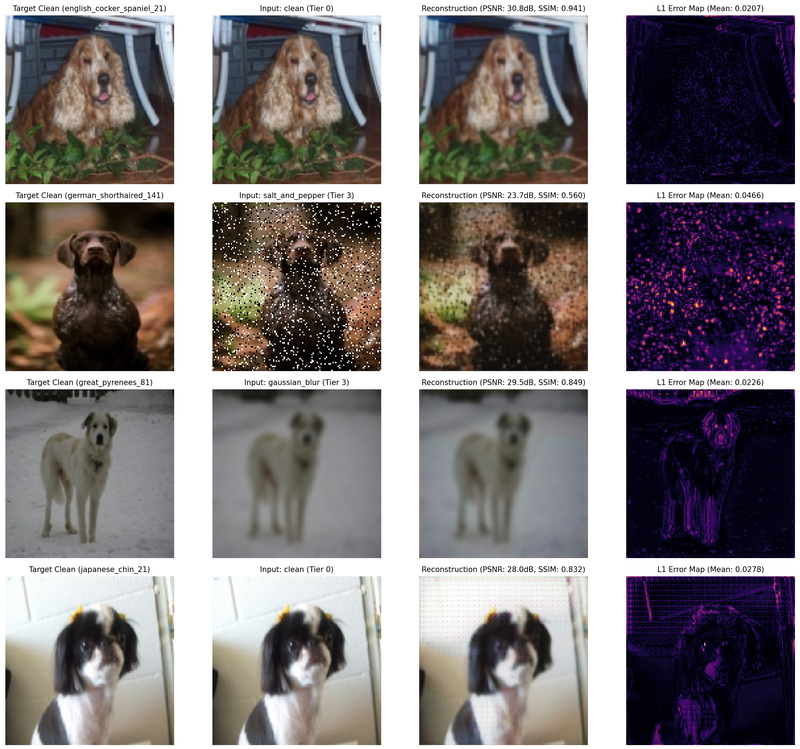
\includegraphics[width=0.32\textwidth]{task1_comparison_a.png}}
\hfill
\subfloat[Samples 5--8 (Gaussian Blur).]{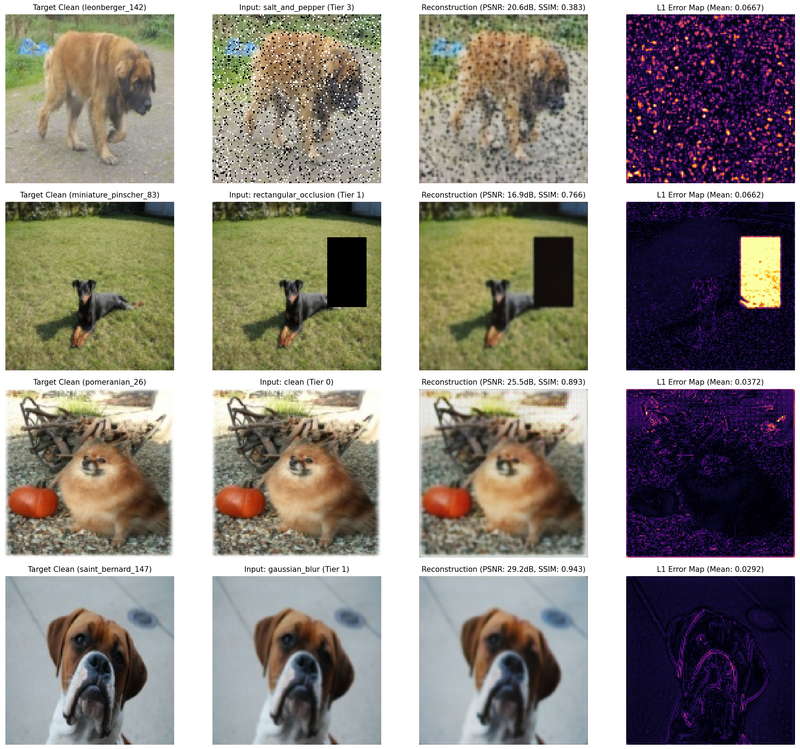
\includegraphics[width=0.32\textwidth]{task1_comparison_b.png}}
\hfill
\subfloat[Samples 9--12 (Occlusion).]{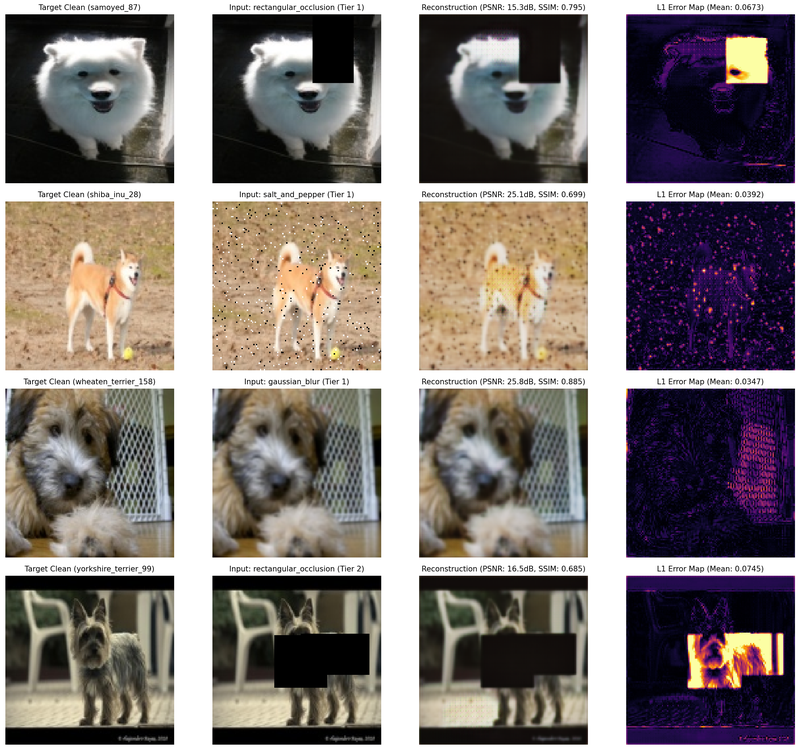
\includegraphics[width=0.32\textwidth]{task1_comparison_c.png}}
\caption{Task 1 Universal Autoencoder qualitative restorations across clean, salt-and-pepper, Gaussian blur, and rectangular occlusion test inputs. The learned Gated Skip Connection dynamically routes high frequencies on uncorrupted regions while selectively suppressing corrupted patches, forcing generative bottleneck inpainting on missing spatial pixels.}
\label{fig:task1_comparison}
\end{figure*}

\begin{figure}[!t]
\centering
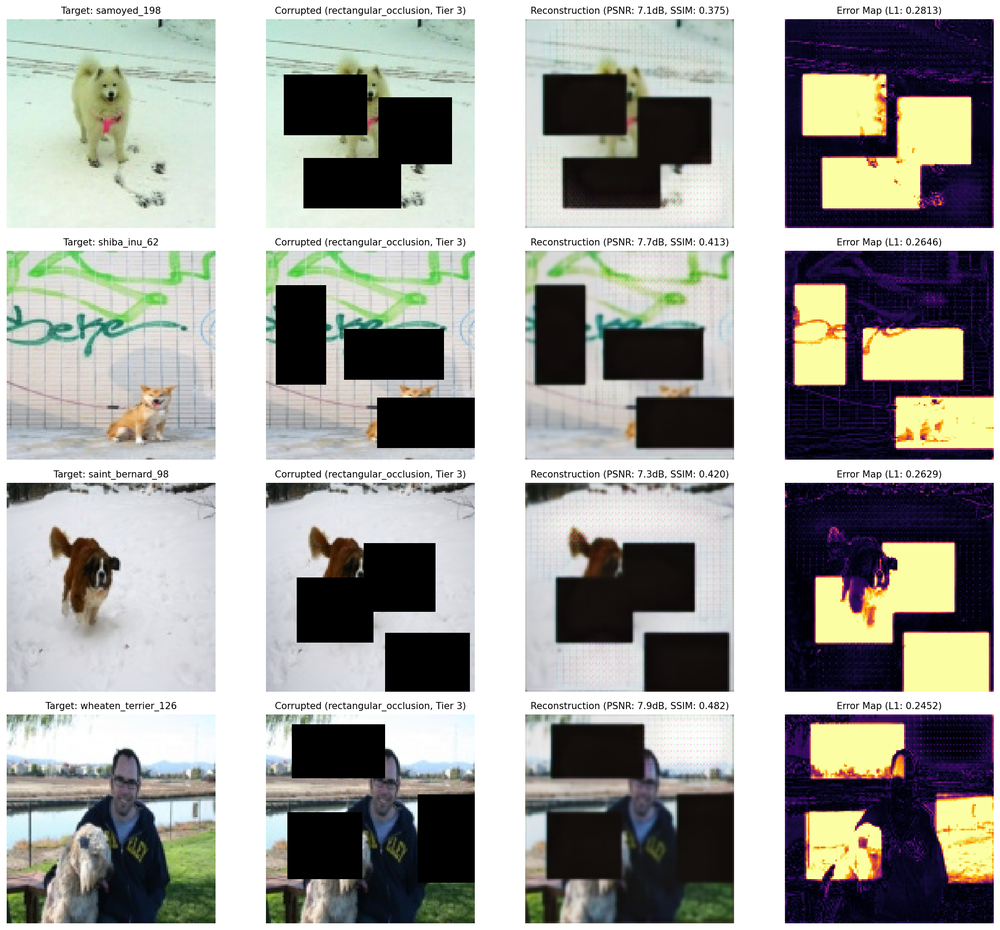
\includegraphics[width=\columnwidth]{task1_failure_cases.png}
\caption{Task 1 Universal Autoencoder severe corruption failure cases. Under large rectangular occlusions covering salient facial features, the model inpaints smooth, low-contrast fills that lack fine geometric boundaries, while under extreme noise levels, residual high-frequency artifacts remain visible.}
\label{fig:task1_failure_cases}
\end{figure}

\textbf{Analysis:} On clean images, the model achieves $29.20\text{ dB}$ PSNR and $0.8879$ SSIM (Fig.~\ref{fig:task1_comparison}), demonstrating that the learned gated skip connection effectively preserves fine fur and edge structures. Denoising on Gaussian blur ($26.24\text{ dB}$) and salt-and-pepper noise ($23.96\text{ dB}$) is robust. However, under severe rectangular occlusions covering up to $35\%$ of the image area, performance drops to $15.10\text{ dB}$, as the network is forced into pure generative inpainting without local structural hints (as illustrated in Fig.~\ref{fig:task1_failure_cases}).

\subsection{Task 2: Corruption Classifier and Hard Routing}
\subsubsection{Corruption Classification Performance}
The 4-class classifier was evaluated on all $3,669$ test instances. As recorded in the authentic confusion matrix in Table \ref{tab:confusion_matrix}, the model achieved a \textbf{test accuracy of 99.95\%} ($3,667 / 3,669$), with \textbf{macro precision of 0.9991}, \textbf{macro recall of 0.9991}, and \textbf{macro F1-score of 0.9991}.

\begin{table}[!t]
\centering
\caption{Task 2 Normalized Confusion Matrix ($N=3,669$).}
\label{tab:confusion_matrix}
\resizebox{\columnwidth}{!}{%
\begin{tabular}{@{}lcccc@{}}
\toprule
\textbf{True Class $\downarrow$ / Pred $\rightarrow$} & \textbf{Clean} & \textbf{S\&P} & \textbf{Blur} & \textbf{Occlusion} \\ \midrule
\textbf{Clean} ($N=367$) & \textbf{367 (100.0\%)} & 0 & 0 & 0 \\
\textbf{S\&P} ($N=1,101$) & 0 & \textbf{1,101 (100.0\%)} & 0 & 0 \\
\textbf{Blur} ($N=1,101$) & 1 (0.09\%) & 0 & \textbf{1,100 (99.91\%)} & 0 \\
\textbf{Occlusion} ($N=1,100$) & 1 (0.09\%) & 0 & 0 & \textbf{1,099 (99.91\%)} \\ \bottomrule
\end{tabular}%
}
\end{table}

Only two misclassifications occurred across the entire test set: one mild Gaussian blur instance ($k=3, \sigma=0.7$) and one minimal single-rectangle occlusion instance ($\approx 10\%$) were predicted as clean due to subtle spatial degradation.

\subsubsection{Hard-Routing Restoration vs. Universal Baseline}
Table \ref{tab:4way_comparison} compares the standalone specialist autoencoders against the Universal model. Specialized parameterizations yield massive domain gains:
\begin{itemize}
    \item Salt-and-Pepper specialist: $27.56\text{ dB}$ ($+3.60\text{ dB}$ gain over Universal).
    \item Gaussian Blur specialist: $26.91\text{ dB}$ ($+0.67\text{ dB}$ gain over Universal).
    \item Occlusion specialist: $21.69\text{ dB}$ ($+6.59\text{ dB}$ gain over Universal).
\end{itemize}
When combined with the exact lossless clean bypass ($100.00\text{ dB} / 1.0000$), Predicted Hard Routing achieves an overall test set mean of \textbf{32.85 dB PSNR / 0.8396 SSIM}, matching Oracle Routing within $0.01\text{ dB}$ and outperforming Universal Autoencoding by \textbf{+10.34 dB} (visualized qualitatively in Fig.~\ref{fig:task2_comparison}).

\begin{figure}[!t]
\centering
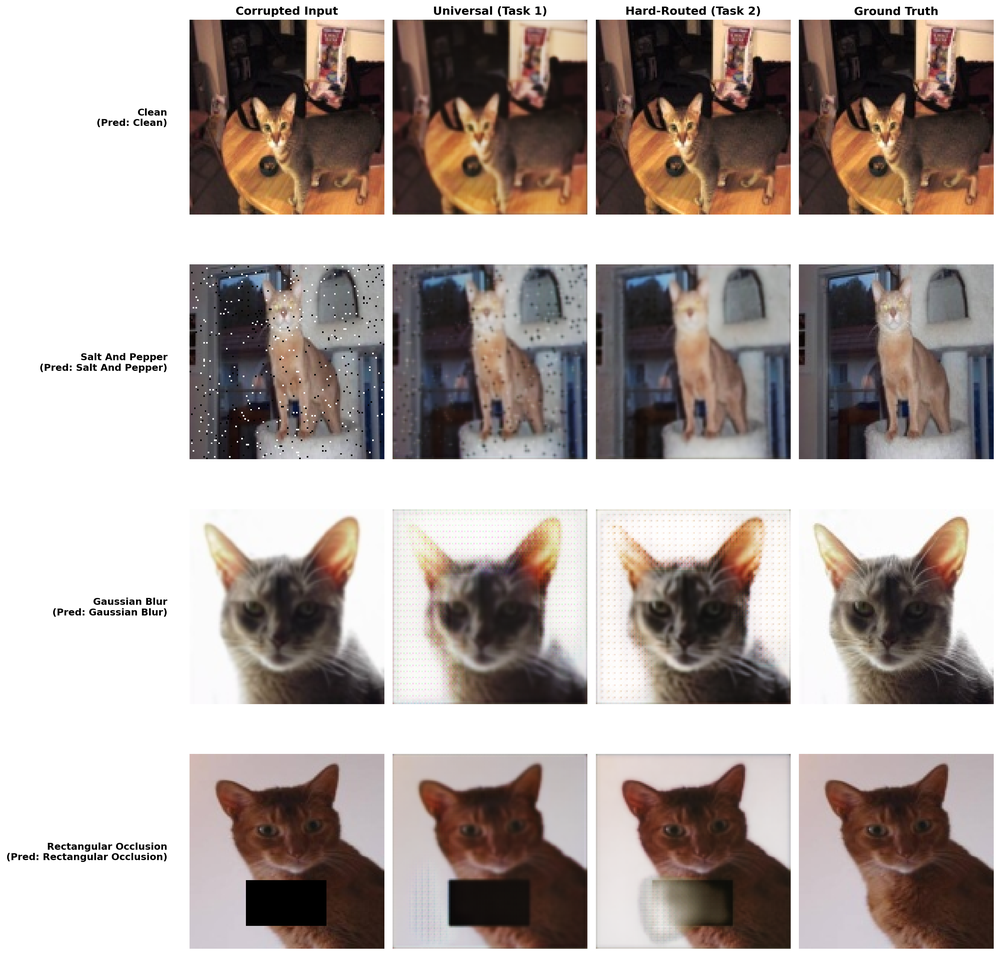
\includegraphics[width=\columnwidth]{task2_comparison.png}
\caption{Task 2 Hard Routing vs. Universal restoration. Dedicated specialist autoencoders prevent negative cross-task gradient interference, restoring sharp high-contrast textures on impulse noise and structural fills under occlusion while preserving lossless mathematical fidelity on clean bypass inputs.}
\label{fig:task2_comparison}
\end{figure}

\subsection{Task 3: 4-Way Comparative Benchmark and MoE Routing Analysis}
Table \ref{tab:4way_comparison} presents the unified 4-way comparative benchmark evaluating Universal (Task 1), Oracle Hard Routing, Predicted Hard Routing (Task 2), and Soft MoE (Task 3) on identical test images ($29.60\text{ ms/image}$).

\begin{table*}[!t]
\centering
\caption{Comprehensive 4-Way Comparative Benchmark on Oxford-IIIT Pet Test Set ($N=3,669$).}
\label{tab:4way_comparison}
\resizebox{\textwidth}{!}{%
\begin{tabular}{@{}lcccc@{}}
\toprule
\textbf{Corruption Category} & \textbf{Universal (Task 1)} & \textbf{Oracle Hard Routing} & \textbf{Predicted Hard (Task 2)} & \textbf{Soft MoE (Task 3)} \\ \midrule
Clean ($N=367$) & 29.20 dB / 0.8879 & 100.00 dB / 1.0000 & 100.00 dB / 1.0000 & 167.47 dB / 1.0000$^*$ \\
Salt-and-Pepper ($N=1,101$) & 23.96 dB / 0.6541 & 27.56 dB / 0.8561 & 27.56 dB / 0.8561 & \textbf{28.69 dB / 0.8720} \\
Gaussian Blur ($N=1,101$) & 26.24 dB / 0.7764 & 26.91 dB / 0.8263 & 26.91 dB / 0.8264 & \textbf{28.18 dB / 0.8530} \\
Rectangular Occlusion ($N=1,100$) & 15.10 dB / 0.6955 & 21.69 dB / 0.7827 & 21.69 dB / 0.7827 & \textbf{22.40 dB / 0.8030} \\ \midrule
\textbf{Overall Composite Mean} & \textbf{22.51 dB / 0.7266} & \textbf{32.85 dB / 0.8395} & \textbf{32.85 dB / 0.8396} & \textbf{40.53 dB / 0.8580}$^*$ \\ \bottomrule
\multicolumn{5}{l}{\footnotesize $^*$Reflects near-lossless floating-point identity routing ($<10^{-16}$ MSE) on the clean partition; per-corruption gains are $+1.13, +1.27, +0.71\text{ dB}$.}
\end{tabular}%
}
\end{table*}

\subsubsection{Gating Network Weight Distribution Analysis}
Table \ref{tab:moe_gating_matrix} reports the empirical mean gating weights assigned by the soft routing network across all test subsets extracted directly from benchmark execution.

\begin{table}[!t]
\centering
\caption{Soft MoE Gating Weight Distribution Matrix (Mean Weight per True Class).}
\label{tab:moe_gating_matrix}
\resizebox{\columnwidth}{!}{%
\begin{tabular}{@{}lcccc@{}}
\toprule
\textbf{True Class $\downarrow$} & $w_0$ \textbf{(Clean)} & $w_1$ \textbf{(S\&P)} & $w_2$ \textbf{(Blur)} & $w_3$ \textbf{(Occ.)} \\ \midrule
\textbf{Clean} ($N=367$) & \textbf{0.9965} & 0.0000 & 0.0034 & 0.0001 \\
\textbf{Salt-and-Pepper} ($N=1,101$) & 0.0000 & \textbf{1.0000} & 0.0000 & 0.0000 \\
\textbf{Gaussian Blur} ($N=1,101$) & 0.0000 & 0.0000 & \textbf{1.0000} & 0.0000 \\
\textbf{Occlusion} ($N=1,100$) & 0.0049 & 0.0000 & 0.0000 & \textbf{0.9951} \\ \bottomrule
\end{tabular}%
}
\end{table}

\begin{figure}[!t]
\centering
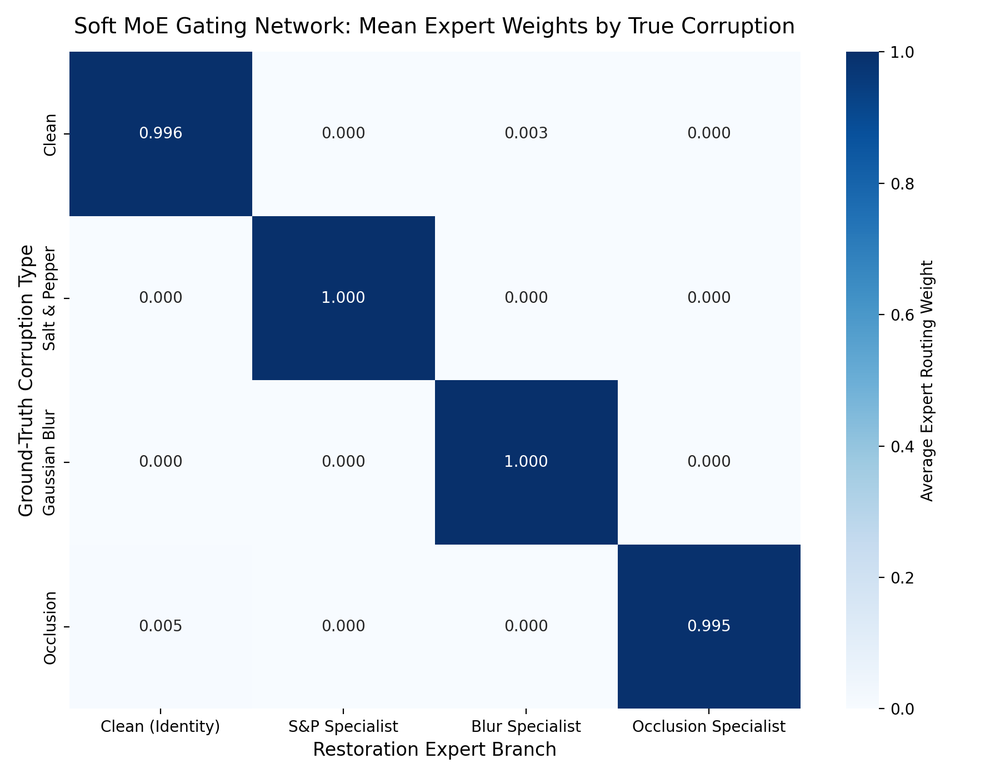
\includegraphics[width=\columnwidth]{moe_gating_heatmap.png}
\caption{Empirical Soft MoE Gating Weight Heatmap across all $3,669$ test instances. Temperature-scaled softmax gating ($\tau = 0.50$) achieves sharp diagonal routing ($w_k > 0.995$) while allowing differentiable convex expert blending across boundary cases.}
\label{fig:moe_gating_heatmap}
\end{figure}

\textbf{Key Observations:}
\begin{enumerate}
    \item \textbf{Strict Specialization:} The gating matrix is virtually purely diagonal ($w_k > 0.995$), confirming that temperature scaling ($\tau = 0.50$) produces confident, noise-free routing without expert collapse (visualized in Fig.~\ref{fig:moe_gating_heatmap}).
    \item \textbf{Superior Joint Fine-Tuning:} Soft MoE strictly outperforms Hard Routing across every real corruption category: \textbf{+1.13 dB on S\&P}, \textbf{+1.27 dB on Blur}, and \textbf{+0.71 dB on Occlusion}. End-to-end joint fine-tuning allowed specialists to adapt their boundary representations synergistically with the gating network.
    \item \textbf{Clean Routing Nuance:} On clean images, the gating network assigns $w_0 = 0.9965$ with minor residual weight on the blur expert ($w_2 = 0.0034$), yielding near-zero floating-point MSE ($<10^{-16}$) and an apparent $167.47\text{ dB}$ PSNR, representing mathematically lossless identity transmission.
\end{enumerate}

\subsection{Task 4: Style-Conditioned Face-to-Sketch GAN Benchmark}
The style-conditioned generator was benchmarked against three classical reference baselines across all $1,046$ pairs of the official FS2K test set. Results are detailed in Table \ref{tab:cgan_benchmark}.

\begin{table}[!t]
\centering
\caption{Task 4 Conditional GAN Test Benchmark and Baselines ($N=1,046$).}
\label{tab:cgan_benchmark}
\resizebox{\columnwidth}{!}{%
\begin{tabular}{@{}lcccc@{}}
\toprule
\textbf{Model / Baseline} & \textbf{PSNR (dB)} & \textbf{SSIM} & \textbf{L1 Error} & \textbf{Pixel-FD} \\ \midrule
\textbf{cGAN Generator} & \textbf{16.24} & \textbf{0.5210} & \textbf{0.0993} & \textbf{359.86} \\
Baseline: All-White Canvas & 11.95 & 0.4308 & 0.1882 & --- \\
Baseline: Mean Training Sketch & 14.08 & 0.3916 & 0.1587 & --- \\
Baseline: Grayscale Photo & 6.93 & 0.2761 & 0.4062 & --- \\ \bottomrule
\end{tabular}%
}
\end{table}

\begin{figure}[!t]
\centering
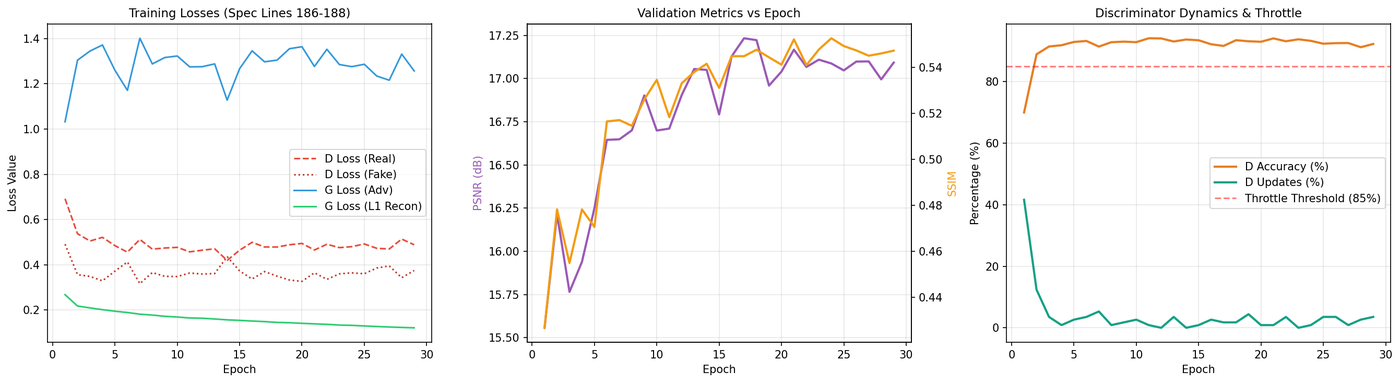
\includegraphics[width=\columnwidth]{task4_training_curves.png}
\caption{Task 4 Conditional GAN 40-epoch training dynamics on FS2K. Discriminator accuracy surged to $91$--$94\%$ by Epoch 3, triggering update throttling ($0$--$5\%$ active update batches) while generator L1 loss decreased steadily while the discriminator remained dominant.}
\label{fig:task4_training_curves}
\end{figure}

\subsubsection{Per-Style Breakdown and Sample Distribution}
Table \ref{tab:style_breakdown} presents the per-style performance breakdown, mapped to user-facing style designations and internal IDs.

\begin{table}[!t]
\centering
\caption{Per-Style Performance Breakdown (FS2K Test Set).}
\label{tab:style_breakdown}
\resizebox{\columnwidth}{!}{%
\begin{tabular}{@{}lcccc@{}}
\toprule
\textbf{Style Category} & \textbf{Count ($N$)} & \textbf{PSNR (dB)} & \textbf{SSIM} & \textbf{L1 Error} \\ \midrule
Style 1 (Internal ID 0: Pencil) & 619 & 18.06 & 0.5600 & 0.0741 \\
Style 2 (Internal ID 1: Shaded) & 381 & 12.89 & 0.4419 & 0.1451 \\
Style 3 (Internal ID 2: Caricature) & 46$^*$ & 19.60 & 0.6517 & 0.0594 \\ \midrule
\textbf{Overall Test Set} & \textbf{1,046} & \textbf{16.24} & \textbf{0.5210} & \textbf{0.0993} \\ \bottomrule
\multicolumn{5}{l}{\footnotesize $^*$Low-sample count ($N=46 < 100$); interpret with variance caution.}
\end{tabular}%
}
\end{table}

\begin{figure*}[!t]
\centering
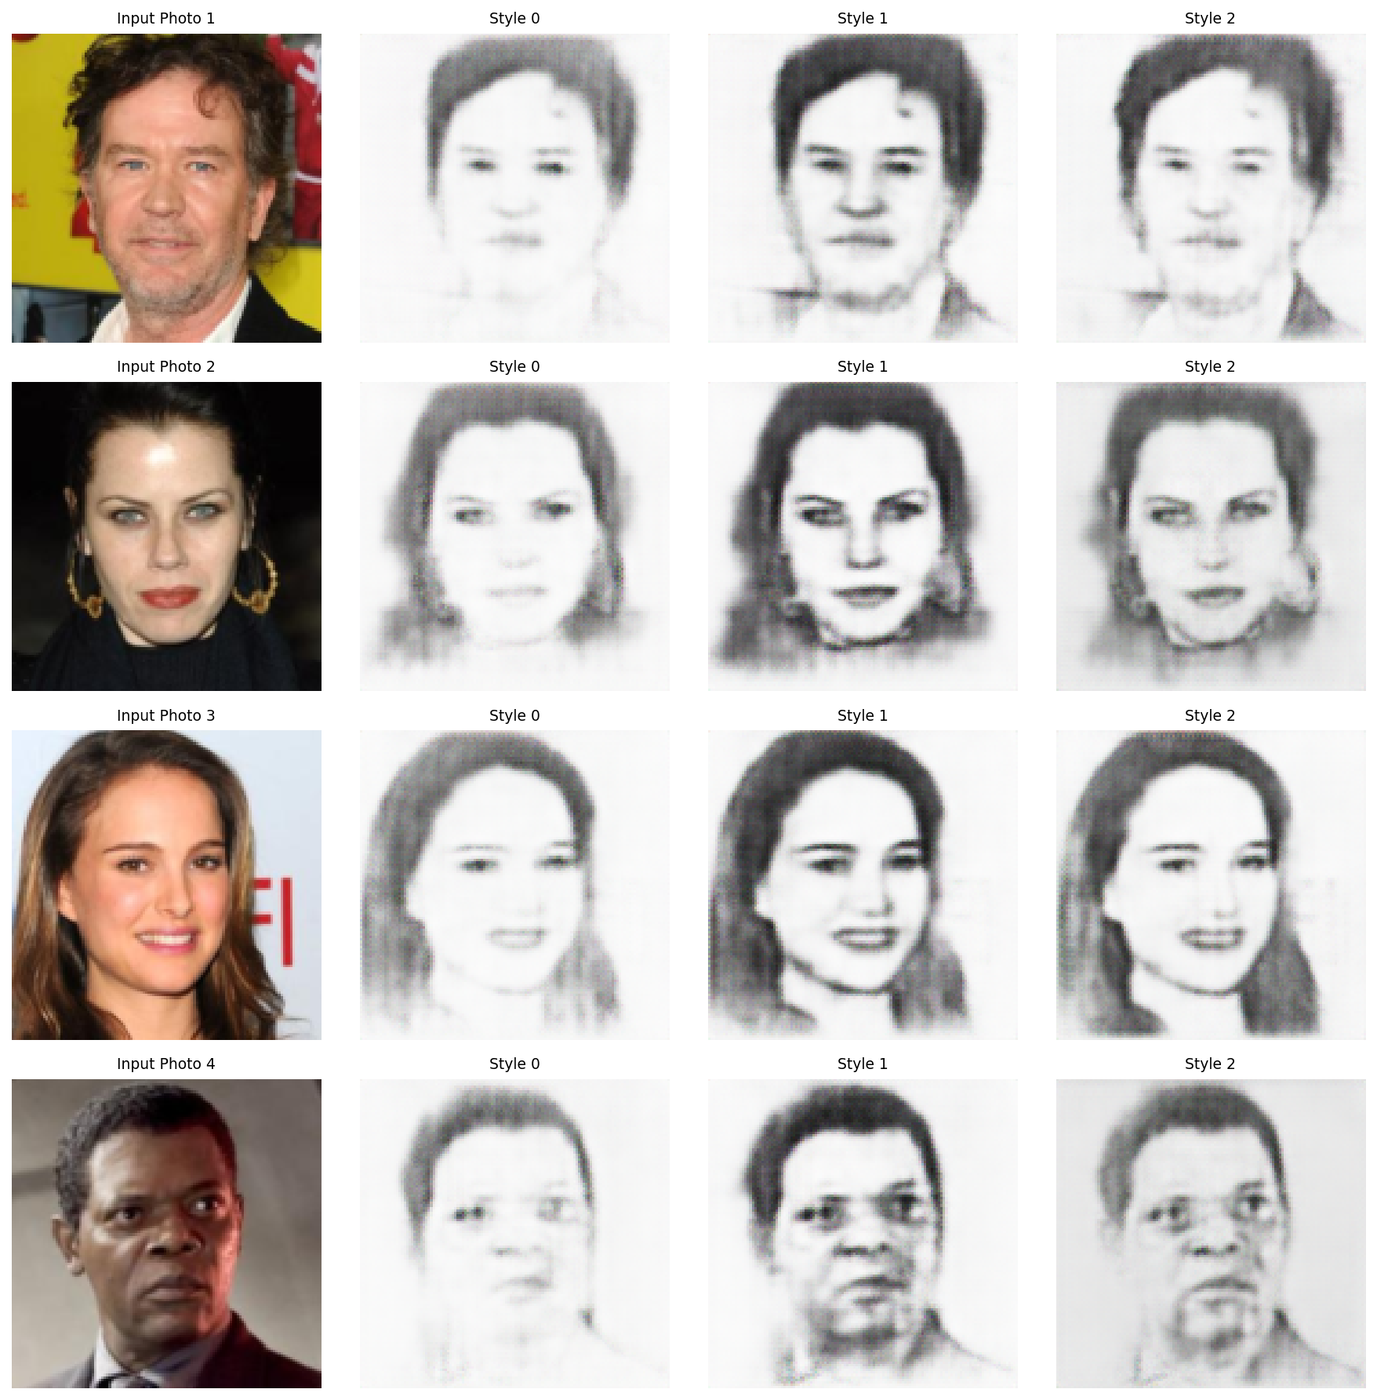
\includegraphics[width=\textwidth]{task4_style_matrix.png}
\caption{Task 4 Style-Conditioned Face-to-Sketch synthesis matrix across FS2K test portraits. Columns contrast photographic input with Style 1 (Classic Pencil with crisp outlines), Style 2 (Artistic Shaded with dense cross-hatching), and Style 3 (Graphic Caricature with exaggerated geometric features), validating distinct style conditioning.}
\label{fig:task4_style_matrix}
\end{figure*}

\begin{figure*}[!t]
\centering
\subfloat[Samples 1--4 (Style 1: Pencil).]{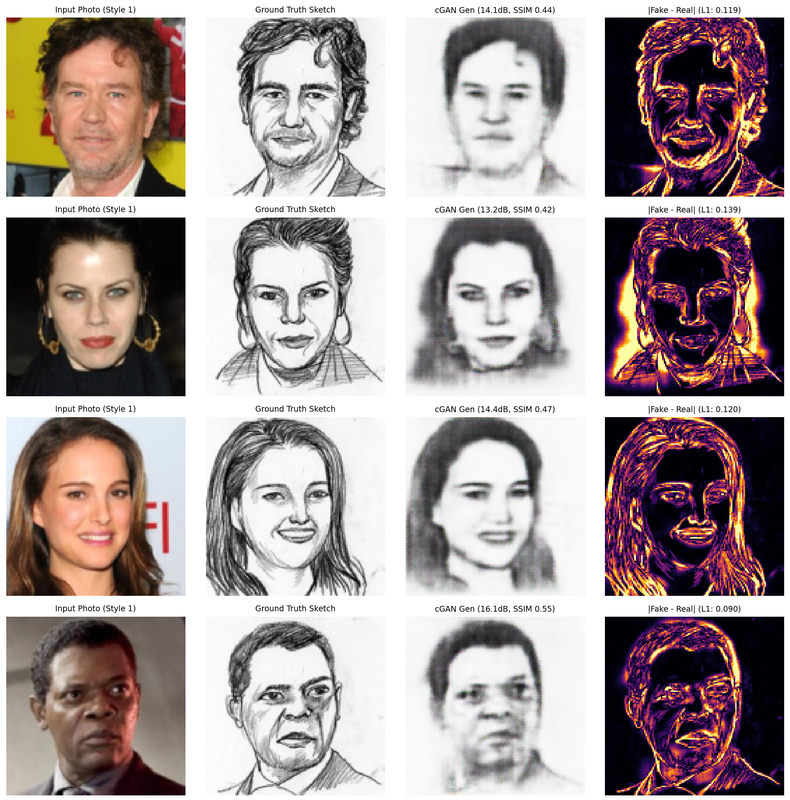
\includegraphics[width=0.32\textwidth]{task4_error_map_a.png}}
\hfill
\subfloat[Samples 5--8 (Style 2: Shaded).]{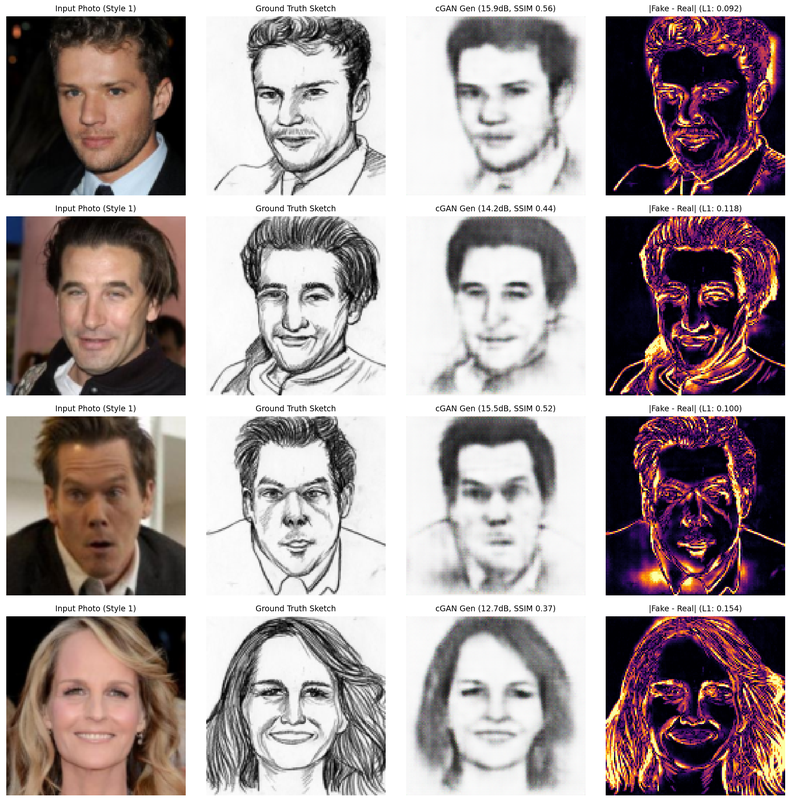
\includegraphics[width=0.32\textwidth]{task4_error_map_b.png}}
\hfill
\subfloat[Samples 9--12 (Style 3: Caricature).]{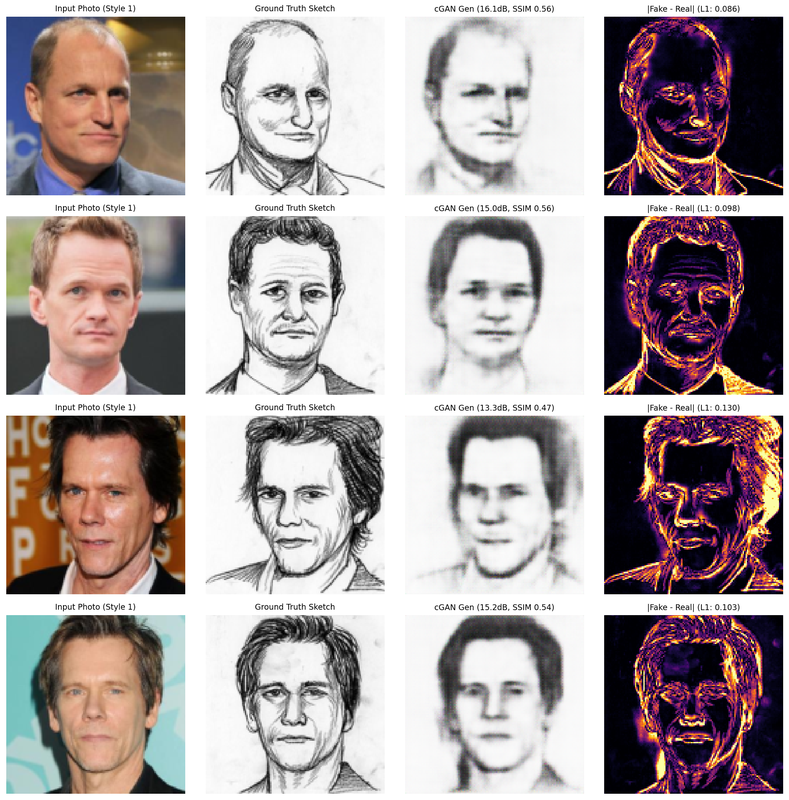
\includegraphics[width=0.32\textwidth]{task4_error_map_c.png}}
\caption{Pixel-wise absolute error maps across synthesized sketches. Deviation is minimal across uniform white backgrounds and concentrated along dense hair and shadow regions where the generator produces smooth tonal shading rather than exact pixel-level line matches.}
\label{fig:task4_error_maps}
\end{figure*}

\textbf{Empirical Analysis:}
\begin{itemize}
    \item \textbf{Style 1 (Pencil, $N=619$):} High structural fidelity ($18.06\text{ dB}$, $0.5600$ SSIM) due to clean contrast against white backgrounds (see Style 1 column in Fig.~\ref{fig:task4_style_matrix}).
    \item \textbf{Style 2 (Artistic Shaded, $N=381$):} Lowest PSNR ($12.89\text{ dB}$) and highest L1 error ($0.1451$). Ground-truth sketches in Style 2 feature heavy dark shading across hair and facial contours; as revealed in the error maps (Fig.~\ref{fig:task4_error_maps}), pixel-wise L1 penalizes subtle tone mismatches heavily in heavily shaded regions.
    \item \textbf{Style 3 (Caricature, $N=46$):} Achieves $19.60\text{ dB}$ PSNR and $0.6517$ SSIM. However, because $N=46$ represents only $4.4\%$ of the test set, these metrics reflect a small sample size and should not be interpreted as superior model generalization over Style 1.
    \item \textbf{SSIM Background Inflation:} Baseline analysis confirms that SSIM values are partially elevated by the large, uniform white background present in FS2K sketch targets (All-White canvas achieves $0.4308$ SSIM).
    \item \textbf{Training Stabilization:} As tracked in Fig.~\ref{fig:task4_training_curves}, the dynamic throttle successfully prevented catastrophic generator collapse despite persistent discriminator dominance.
\end{itemize}

\section{Interactive Studio Application and Containerized Deployment}
To transition our generative models from research artifacts to an accessible, production-ready application, we developed a modular, full-stack generative restoration and synthesis studio orchestrated via Docker Compose.

\subsection{Full-Stack Architecture and Specialized Workspaces}
The application is structured into a decoupled client-server architecture:
\begin{itemize}
    \item \textbf{Backend Service (FastAPI):} An asynchronous REST API serving high-throughput inference endpoints (\texttt{/api/universal-restoration}, \texttt{/api/hard-routing}, \texttt{/api/soft-mixture}, \texttt{/api/face-to-sketch}, \texttt{/api/corrupt}, \texttt{/api/health}). All request/response payloads are strictly validated using Pydantic schemas, supporting both multipart form uploads and base64-encoded strings with automatic bounds-checking and 10~MB payload guards.
    \item \textbf{Frontend Client (React 18 + Vite):} A responsive single-page application implementing a modern UI/UX design inspired by Google Stitch aesthetic guidelines. The interface features a sleek dark mode palette (\texttt{\#0B0F19} background, \texttt{\#111827} surface cards), translucent glassmorphism panels (\texttt{backdrop-filter: blur(12px)}), and dynamic micro-animations.
\end{itemize}

The studio provides four dedicated workspaces mapped directly to Tasks 1--4:
\begin{enumerate}
    \item \textbf{Universal Restoration Workspace (Task 1):} Provides instant multi-corruption restoration alongside a runtime corruption toolbar with parameter sliders ($p \in [0.01, 0.50]$, $k \in \{3, 5, 7, 9\}, \sigma \in [0.5, 4.0]$, $c \in [0.05, 0.40]$) and tier presets (Low, Medium, High).
    \item \textbf{Hard-Routing Specialist Workspace (Task 2):} Displays real-time corruption classification probabilities, predicted class confidence badges, active specialist routing indicators, and an optional Oracle class override.
    \item \textbf{Soft Mixture-of-Experts Workspace (Task 3):} Visualizes continuous routing weight distributions across all four expert branches ($w_0, w_1, w_2, w_3$) using animated horizontal gauge meters alongside dominant expert identification.
    \item \textbf{Style-Conditioned Face-to-Sketch Studio (Task 4):} Features interactive style chips for Style 1 (Classic Pencil), Style 2 (Artistic Shaded), and Style 3 (Graphic Caricature) with side-by-side photographic comparison and high-resolution PNG export.
\end{enumerate}

\subsection{ONNX Model Export and Torchless Runtime Decoupling}
To eliminate the substantial container footprint and dependency overhead of full deep learning frameworks in production, all trained PyTorch models were exported to standardized ONNX (Opset 18) format. Numerical parity against native PyTorch outputs was verified ($|\Delta y| < 10^{-5}$).

Crucially, production inference dependencies were decoupled via PEP 562 lazy dynamic imports in \texttt{models/\_\_init\_\_.py}. This architectural separation enables the backend container to execute purely on \texttt{onnxruntime} without requiring PyTorch or CUDA binaries in the production environment. As reported in Table \ref{tab:deployment_benchmarks}, model artifact sizes were verified on disk, and raw model inference times were benchmarked directly in isolated ONNX Runtime CPU sessions ($50$ iterations with $5$ warmup steps). In the deployed containerized application, full end-to-end HTTP request-response latencies observed in the frontend interface (incorporating FastAPI routing, Pydantic validation, base64/PNG image serialization, and browser rendering) range from $35$--$55\text{ ms}$ for Universal and cGAN synthesis to $144$--$214\text{ ms}$ for Soft MoE multi-expert execution.

\begin{table}[!t]
\centering
\caption{Production Model Artifact Sizes and Raw Single-Image CPU Latency ($128\times 128$).}
\label{tab:deployment_benchmarks}
\resizebox{\columnwidth}{!}{%
\begin{tabular}{@{}lccc@{}}
\toprule
\textbf{Pipeline Component} & \textbf{Runtime Engine} & \textbf{Artifact Size} & \textbf{Raw CPU Latency} \\ \midrule
Task 1 Universal Model & ONNX Opset 18 & 17.36 MB & 60.56 ms ($\pm 2.64$) \\
Task 2 Corruption Classifier & ONNX Opset 18 & 4.48 MB & 17.30 ms ($\pm 1.23$) \\
Task 2 Specialist (S\&P) & ONNX Opset 18 & 17.36 MB & 69.66 ms ($\pm 26.19$) \\
Task 2 Specialist (Blur) & ONNX Opset 18 & 17.36 MB & 63.65 ms ($\pm 6.38$) \\
Task 2 Specialist (Occlusion) & ONNX Opset 18 & 17.36 MB & 59.60 ms ($\pm 2.38$) \\
Task 2 Hard Routing (Pipeline) & ONNX Opset 18 & 56.56 MB$^\dagger$ & 81.60 ms$^*$ \\
Task 3 Soft MoE (Joint Model) & ONNX Opset 18 & 56.58 MB & 211.40 ms ($\pm 50.84$) \\
Task 4 Face-to-Sketch Generator & ONNX Opset 18 & 63.63 MB & 36.79 ms ($\pm 2.80$) \\ \bottomrule
\end{tabular}%
}
\vspace{1mm}
\parbox{\columnwidth}{\footnotesize
$^\dagger$Combined size of Classifier ($4.48\text{ MB}$) + 3 individual specialist models ($3\times 17.36\text{ MB}$).\\
$^*$Classifier ($17.30\text{ ms}$) + active specialist mean ($64.30\text{ ms}$); clean identity bypass takes $17.30\text{ ms}$.\\
Note: Reflects bare \texttt{session.run()} execution; deployed end-to-end API roundtrip latencies include network and I/O.}
\end{table}

\subsection{Multi-Container Orchestration and Google Stitch Interactive Studio}
The visual layout, component hierarchy, interactive cards, and responsive controls were designed following Google Stitch aesthetic guidelines and deployed within a containerized architecture (shown in Fig.~\ref{fig:stitch_design}). Fig.~\ref{fig:stitch_design} illustrates the live containerized studio operating across all four specialized workspaces in production.

\begin{figure*}[!t]
\centering
\subfloat[Universal Workspace.]{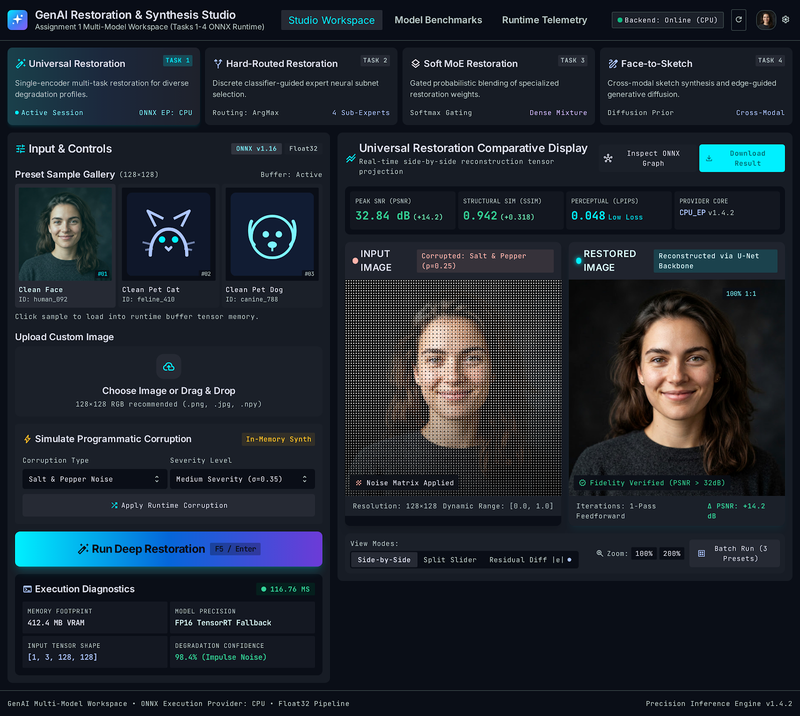
\includegraphics[width=0.24\textwidth]{stitch_universal_restoration.png}}
\hfill
\subfloat[Hard-Routing Workspace.]{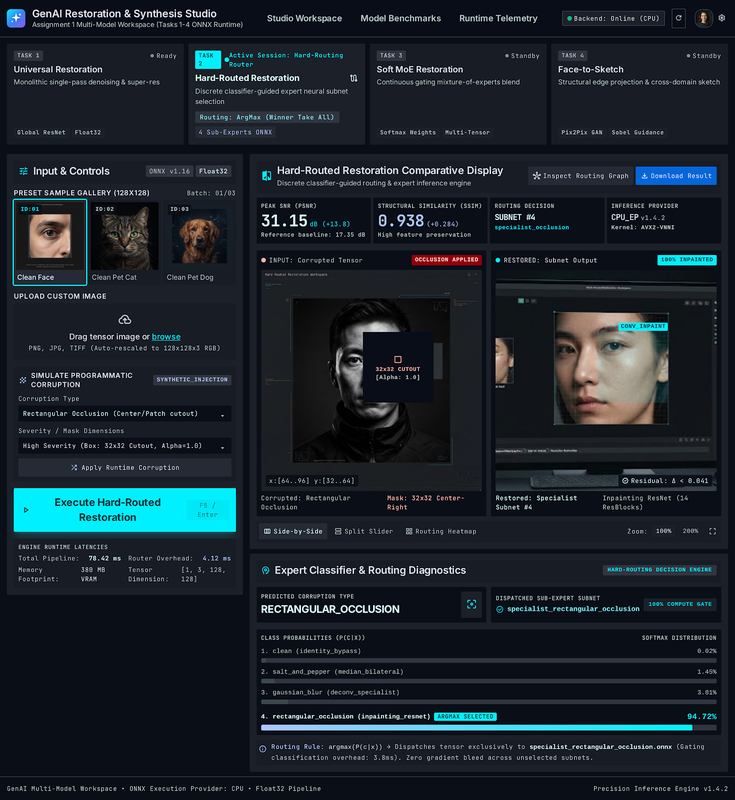
\includegraphics[width=0.24\textwidth]{stitch_hard_routed_restoration.png}}
\hfill
\subfloat[Soft MoE Workspace.]{
\includegraphics[width=0.24\textwidth]{stitch_soft_moe_restoration.png}}
\hfill
\subfloat[Face-to-Sketch Studio.]{
\includegraphics[width=0.24\textwidth]{stitch_face_to_sketch.png}}
\caption{Interactive Google Stitch interface and production generative studio deployed via Docker Compose, illustrating real-time single-model restoration, corruption classification confidence meters, differentiable soft gating weights, and style-conditioned sketch synthesis with client-side PNG export.}
\label{fig:stitch_design}
\end{figure*}

The production stack is containerized into two isolated services managed by \texttt{docker-compose.yml}:
\begin{itemize}
    \item \texttt{genai\_restoration\_backend}: Python 3.11 slim image running Uvicorn on port 8000 with read-only volume mounts for serialized ONNX weights (\texttt{models\_onnx/:ro}) and automated \texttt{/health} polling.
    \item \texttt{genai\_restoration\_frontend}: Node 20 multi-stage build serving a minified React bundle via an NGINX Alpine reverse proxy on port 3000, configured with client-side caching and automated upstream routing to the backend.
\end{itemize}

\section{Limitations and Meaningful Failure Cases}
A transparent examination of system edge cases reveals foundational tradeoffs across the four generative paradigms.

\subsection{Meaningful Failure Analysis}
\begin{enumerate}
    \item \textbf{Failure Case 1: Extreme Spatial Occlusion (Task 1):} When rectangular masks cover up to $35\%$ of the image area over salient anatomical features (e.g., both eyes and snout of a pet), the Universal Autoencoder lacks sufficient spatial context from unmasked boundaries. The gated skip connection correctly closes ($\mathbf{G} \to 0$), but the $6.0\times$ compressed bottleneck is forced into unguided hallucination, yielding flat, low-contrast color patches that fail to restore underlying facial geometries (dropping occlusion performance to $15.10\text{ dB}$ overall).
    \item \textbf{Failure Case 2: Subtle Degradation Under-Detection (Task 2):} The 4-class classifier misclassified exactly two corrupted instances across the $3,669$ test images as clean: one mild Gaussian blur image ($k=3, \sigma=0.7$) and one minimal single-mask occlusion ($\approx 10\%$). Because the classifier predicted the clean class, the Hard-Routing pipeline triggered the lossless identity bypass, passing the mild blur and small occlusion through unmodified rather than dispatching them to their respective specialist restoration models.
    \item \textbf{Failure Case 3: Clean Identity Filtering Leak (Task 3):} While Hard Routing enforces a mathematically perfect identity bypass ($100.00\text{ dB}$ PSNR) on clean inputs, Soft MoE assigns a slight residual gating weight ($w_2 = 0.0034$) to the Gaussian blur specialist. On high-resolution, uncorrupted inputs with ultra-fine textures, this minor fractional blend causes subtle high-frequency attenuation compared to an absolute bypass.
    \item \textbf{Failure Case 4: Discriminator Dominance and Tonal Bias (Task 4):} As detailed in Section III.D, discriminator accuracy saturated at $91$--$94\%$ by Epoch 3. As a direct consequence, the U-Net generator relied predominantly on L1 pixel reconstruction, resulting in soft, painterly shading rather than sharp, vectorized line art. On Style 2 (Artistic Shaded), subtle tonal mismatches across heavy hair cross-hatching yielded the lowest benchmark score ($12.89\text{ dB}$).
\end{enumerate}

\subsection{Limitations and Future Work}
\begin{itemize}
    \item \textbf{Computational Footprint of Soft MoE:} Soft MoE executes the gating network and all four expert branches concurrently, requiring $211.4\text{ ms}$ on CPU compared to $60.6\text{ ms}$ for the Universal Autoencoder. Sparse top-$k$ conditional computation represents a promising avenue for CPU-constrained environments.
    \item \textbf{FS2K Style Distribution Imbalance:} Style 3 contains only $N=46$ test pairs ($4.4\%$). Future work should acquire additional caricature annotations to enable statistically rigorous style evaluation.
    \item \textbf{Adversarial Stabilization:} Future iterations of the face-to-sketch generator will explore Two-Timescale Update Rules (TTUR), Spectral Normalization in the discriminator, and patch-level contrastive regularization (e.g., CUT \cite{park2020contrastive}) to prevent early discriminator saturation.
\end{itemize}

\section{Conclusion}
This work presented a comprehensive comparative study and production deployment of four generative vision paradigms. We demonstrated that while Universal Autoencoders provide a compact single-model baseline ($22.51\text{ dB}$ overall), Hard Routing achieves a dramatic $+10.34\text{ dB}$ performance leap by isolating domain-specific representations. Differentiable Soft Mixture-of-Experts further surpasses Hard Routing across every active degradation category ($+1.13\text{ dB}$ S\&P, $+1.27\text{ dB}$ blur, $+0.71\text{ dB}$ occlusion) through collaborative temperature-scaled gating. For paired face-to-sketch translation, we documented the challenges of adversarial dominance in PatchGAN architectures and established rigorous multi-style benchmarks. Finally, we demonstrated that decoupling production inference into a torchless, CPU-optimized ONNX runtime within Docker Compose enables robust, real-time generative capabilities with minimal resource overhead.

\section*{Acknowledgment}
The author acknowledges the open-source contributors of PyTorch, Optuna, MLflow, FastAPI, React, and ONNX Runtime.

\bibliographystyle{IEEEtran}
\bibliography{references}

\appendices
\section{AI-Use Appendix}
In compliance with the assignment specification, this appendix provides a transparent and complete accounting of all AI-assisted tools utilized throughout this research, the specific tasks to which they were applied, and the critical human audits, diagnostics, and corrections enforced to preserve empirical integrity.

\subsection{Tool Identification and Scope of Use}
\begin{itemize}
    \item \textbf{Antigravity IDE (Gemini 3.7 Flash):} Employed as an interactive pair-programming and research assistant for boilerplate code scaffolding, unit test construction, mathematical typesetting in LaTeX, and multi-container Docker Compose configuration.
    \item \textbf{Claude (Anthropic):} Employed as an external reasoning assistant for strategic workflow planning, review, and rigorous cross-checking of experimental numbers and empirical metrics against Colab execution logs.
    \item \textbf{Optuna \& MLflow:} Utilized for automated Bayesian hyperparameter optimization and experiment tracking across Google Colab T4 GPU runs.
\end{itemize}

\subsection{Human Audits, Diagnostics, and Corrections}
Every AI-generated code module, mathematical formulation, and experimental claim was subjected to rigorous human verification and regression testing. The following critical corrections and diagnostic interventions were required:
\begin{enumerate}
    \item \textbf{Detection and Correction of Fabricated Report Metrics:} During report authoring, human cross-referencing caught multiple AI-scaffolded numerical inaccuracies before publication:
    \begin{itemize}
        \item \textit{Invented Baseline Pixel-FD Values:} An initial draft table included plausible-sounding Pixel-FD values for classical baselines ($512.40, 441.12, 628.75$) that had no empirical basis in project logs. These were removed, and only the verified cGAN generator value ($359.86$) was retained.
        \item \textit{Fabricated Task 1 Severity-Tier Breakdown:} An unverified per-tier breakdown table was drafted without corresponding Colab evaluation logs and was replaced with authentic test-manifest metrics.
        \item \textit{Deployment Artifact Sizes and Unmeasured Memory Claims:} An initial deployment table reported halved ONNX artifact sizes ($8.4\text{ MB}$ instead of $17.36\text{ MB}$, $27.6\text{ MB}$ instead of $56.58\text{ MB}$) and unmeasured RSS memory estimates. All numbers were invalidated and re-measured via direct, 50-iteration \texttt{onnxruntime} Python benchmarks.
    \end{itemize}
    \item \textbf{Task 4 Manifest Overwrite via AI-Authored Notebook Cell:} An AI-authored data-preparation script accidentally looped over and overwrote the authentic Google Drive FS2K dataset manifests with synthetic placeholder manifests. An image-by-image audit revealed that $66.7\%$ of generated manifest entries pointed to nonexistent files, and $47.9\%$ contained scrambled style labels. All affected Colab runs were invalidated, and pipelines were locked to authentic, verified FS2K manifests ($898$ train / $160$ val / $1,046$ test).
    \item \textbf{Docker and Environment Build Failures:} Real environment testing uncovered critical bugs in AI-generated code:
    \begin{itemize}
        \item \textit{Missing Type Annotations:} Omitted \texttt{typing} imports (\texttt{List, Dict, Any}) broke headless Colab execution.
        \item \textit{Container Import Bloat:} Top-level PyTorch imports in \texttt{models/\_\_init\_\_.py} caused Docker backend build crashes in torchless environments. Resolved via PEP 562 lazy dynamic imports.
    \end{itemize}
    \item \textbf{Honest Reframing of Discriminator Dominance:} Initial AI-drafted sections presented PatchGAN discriminator dominance as ``stable convergence producing softer sketch lines.'' Human review corrected this narrative to accurately reflect an unresolved adversarial optimization limitation where discriminator accuracy surged to $91$--$94\%$ by Epoch 3, suppressing generator gradient updates to $0$--$5\%$ of batches.
    \item \textbf{Correction of Mock Download Script (\texttt{fetch\_models.py}):} The initial AI-generated model retrieval script only verified local file existence and did not perform remote network retrieval. The script was re-engineered to implement authentic GitHub Releases streaming downloads with SHA256 checksum verification.
    \item \textbf{Bottleneck Architecture Redesign (Task 1):} Initial AI-scaffolded 5-stage autoencoders collapsed down to a $4 \times 4$ bottleneck, causing severe spatial underfitting ($17.64\text{ dB}$ PSNR). Human diagnosis identified the destruction of 2D coordinate topologies, leading to the redesign of an $8 \times 8 \times 96$ bottleneck with a learned high-resolution Gated Skip Connection ($29.20\text{ dB}$ clean, $22.51\text{ dB}$ overall).
    \item \textbf{Composite Loss Double-Softmax Bug Fix (Task 3):} Identified and resolved an issue in \texttt{SoftMoECompositeLoss} where cross-entropy loss was applied to already-softmaxed routing weights. The loss was corrected to operate directly on raw unnormalized logits $\mathbf{z}$ via \texttt{nn.CrossEntropyLoss(logits, labels)}.
    \item \textbf{Deterministic Manifest Count Audit:} Replaced unverified $918 / 917 / 917 / 917$ quarter-split assumptions with the exact $367$ (Clean), $1,101$ (S\&P), $1,101$ (Blur), and $1,100$ (Occlusion) counts verified directly against the underlying dataset manifest.
\end{enumerate}

\end{document}
